\documentclass[border=3pt]{standalone}
% Preâmbulo compartilhado pelos diagramas TikZ da aula 5 de IHC (Processos de Design)
\usepackage[T1]{fontenc}
\usepackage[utf8]{inputenc}
\usepackage{lmodern}
\usepackage{amsmath}
\usepackage{xcolor}
\usepackage{tikz}
\usetikzlibrary{arrows.meta,angles,quotes,decorations.pathmorphing,calc,
                positioning,shapes.geometric,shapes.misc,backgrounds,fit,
                math}

% Paleta (mesma dos SVGs originais)
% Paleta da disciplina de IHC: acento roxo (#755099), da capa do livro.
% (o nome "dblue" é mantido para não alterar todos os diagramas)
\definecolor{dblue}{HTML}{755099}
\definecolor{dorange}{HTML}{B3541E}
\definecolor{dgreen}{HTML}{4A7C59}
\definecolor{dred}{HTML}{9C4B4B}
\definecolor{dcream}{HTML}{F4F1EA}
\definecolor{dshade}{HTML}{DDD7C9}

% Função gaussiana (não normalizada por padrão de escala visual)
\pgfmathdeclarefunction{gauss}{3}{%
  \pgfmathparse{1/(#3*sqrt(2*pi))*exp(-((#1-#2)^2)/(2*#3^2))}%
}

% Estilos comuns (prefixo d... para não colidir com chaves internas do pgf)
\tikzset{
  >={Stealth[length=2mm]},
  dguide/.style={gray!55, dashed, line width=0.4pt},
  daxis/.style={gray!60, line width=0.7pt, ->},
  dbody/.style={fill=black!3, draw=black!80, line width=1pt},
  dacc/.style={draw=dblue, line width=1pt},
  dlbl/.style={black!55, font=\small},
  dsub/.style={black!45, font=\footnotesize},
  dstate/.style={circle, draw=black!80, fill=dcream, line width=1pt,
                 minimum size=17mm, font=\large, inner sep=1pt},
  dobs/.style={circle, draw=black!80, fill=dshade, line width=1pt,
               minimum size=14mm, font=\large, inner sep=1pt},
  dbox/.style={rounded corners=2pt, draw=black!80, fill=dcream, line width=1pt,
               align=center, inner sep=6pt},
  dop/.style={circle, draw=black!80, fill=white, line width=1pt,
              minimum size=6mm, inner sep=0pt, font=\small},
  dtrans/.style={->, dblue, line width=1pt},
  dmeas/.style={->, dorange, line width=1pt},
  dcurve/.style={line width=1pt, dblue},
  dcurveb/.style={line width=1.4pt, dorange},
}

\begin{document}
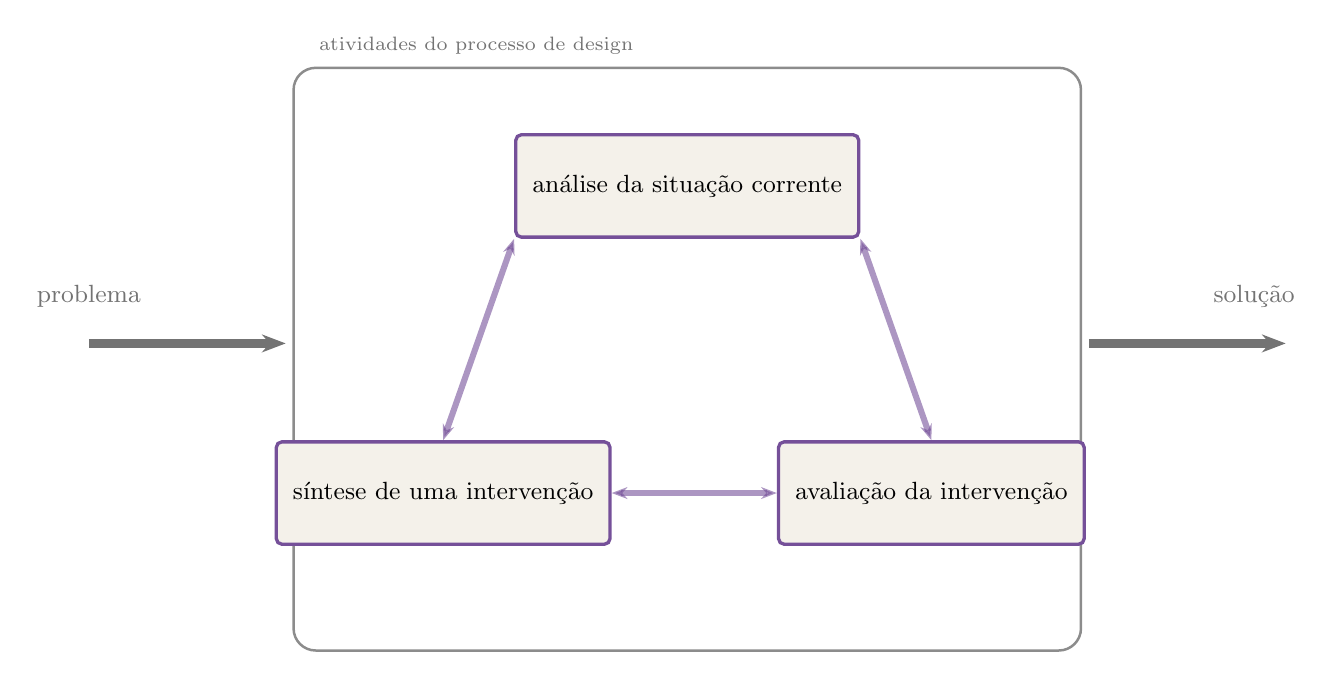
\begin{tikzpicture}[x=1cm,y=1cm,
   act/.style={dbox, minimum width=3.4cm, minimum height=1.3cm, font=\small, draw=dblue, line width=1.2pt}]

  \draw[black!45, rounded corners=8pt, line width=0.9pt] (-1,-3.9) rectangle (9,3.5);
  \node[dlbl, font=\scriptsize, anchor=south west] at (-0.8,3.55) {atividades do processo de design};

  \node[act] (an) at (4,2.0) {análise da situação corrente};
  \node[act] (si) at (0.9,-1.9) {síntese de uma intervenção};
  \node[act] (av) at (7.1,-1.9) {avaliação da intervenção};

  \draw[<->, dblue, line width=2.2pt, opacity=0.6] (an.south west) -- (si.north);
  \draw[<->, dblue, line width=2.2pt, opacity=0.6] (an.south east) -- (av.north);
  \draw[<->, dblue, line width=2.2pt, opacity=0.6] (si.east) -- (av.west);

  \draw[-{Stealth[length=3mm]}, black!55, line width=3.2pt] (-3.6,0) -- (-1.1,0);
  \node[dlbl] at (-3.6,0.6) {problema};
  \draw[-{Stealth[length=3mm]}, black!55, line width=3.2pt] (9.1,0) -- (11.6,0);
  \node[dlbl] at (11.2,0.6) {solução};


\end{tikzpicture}
\end{document}
